\section{Differentialrechnung}
\subsection{Einleitung}
\begin{center}
    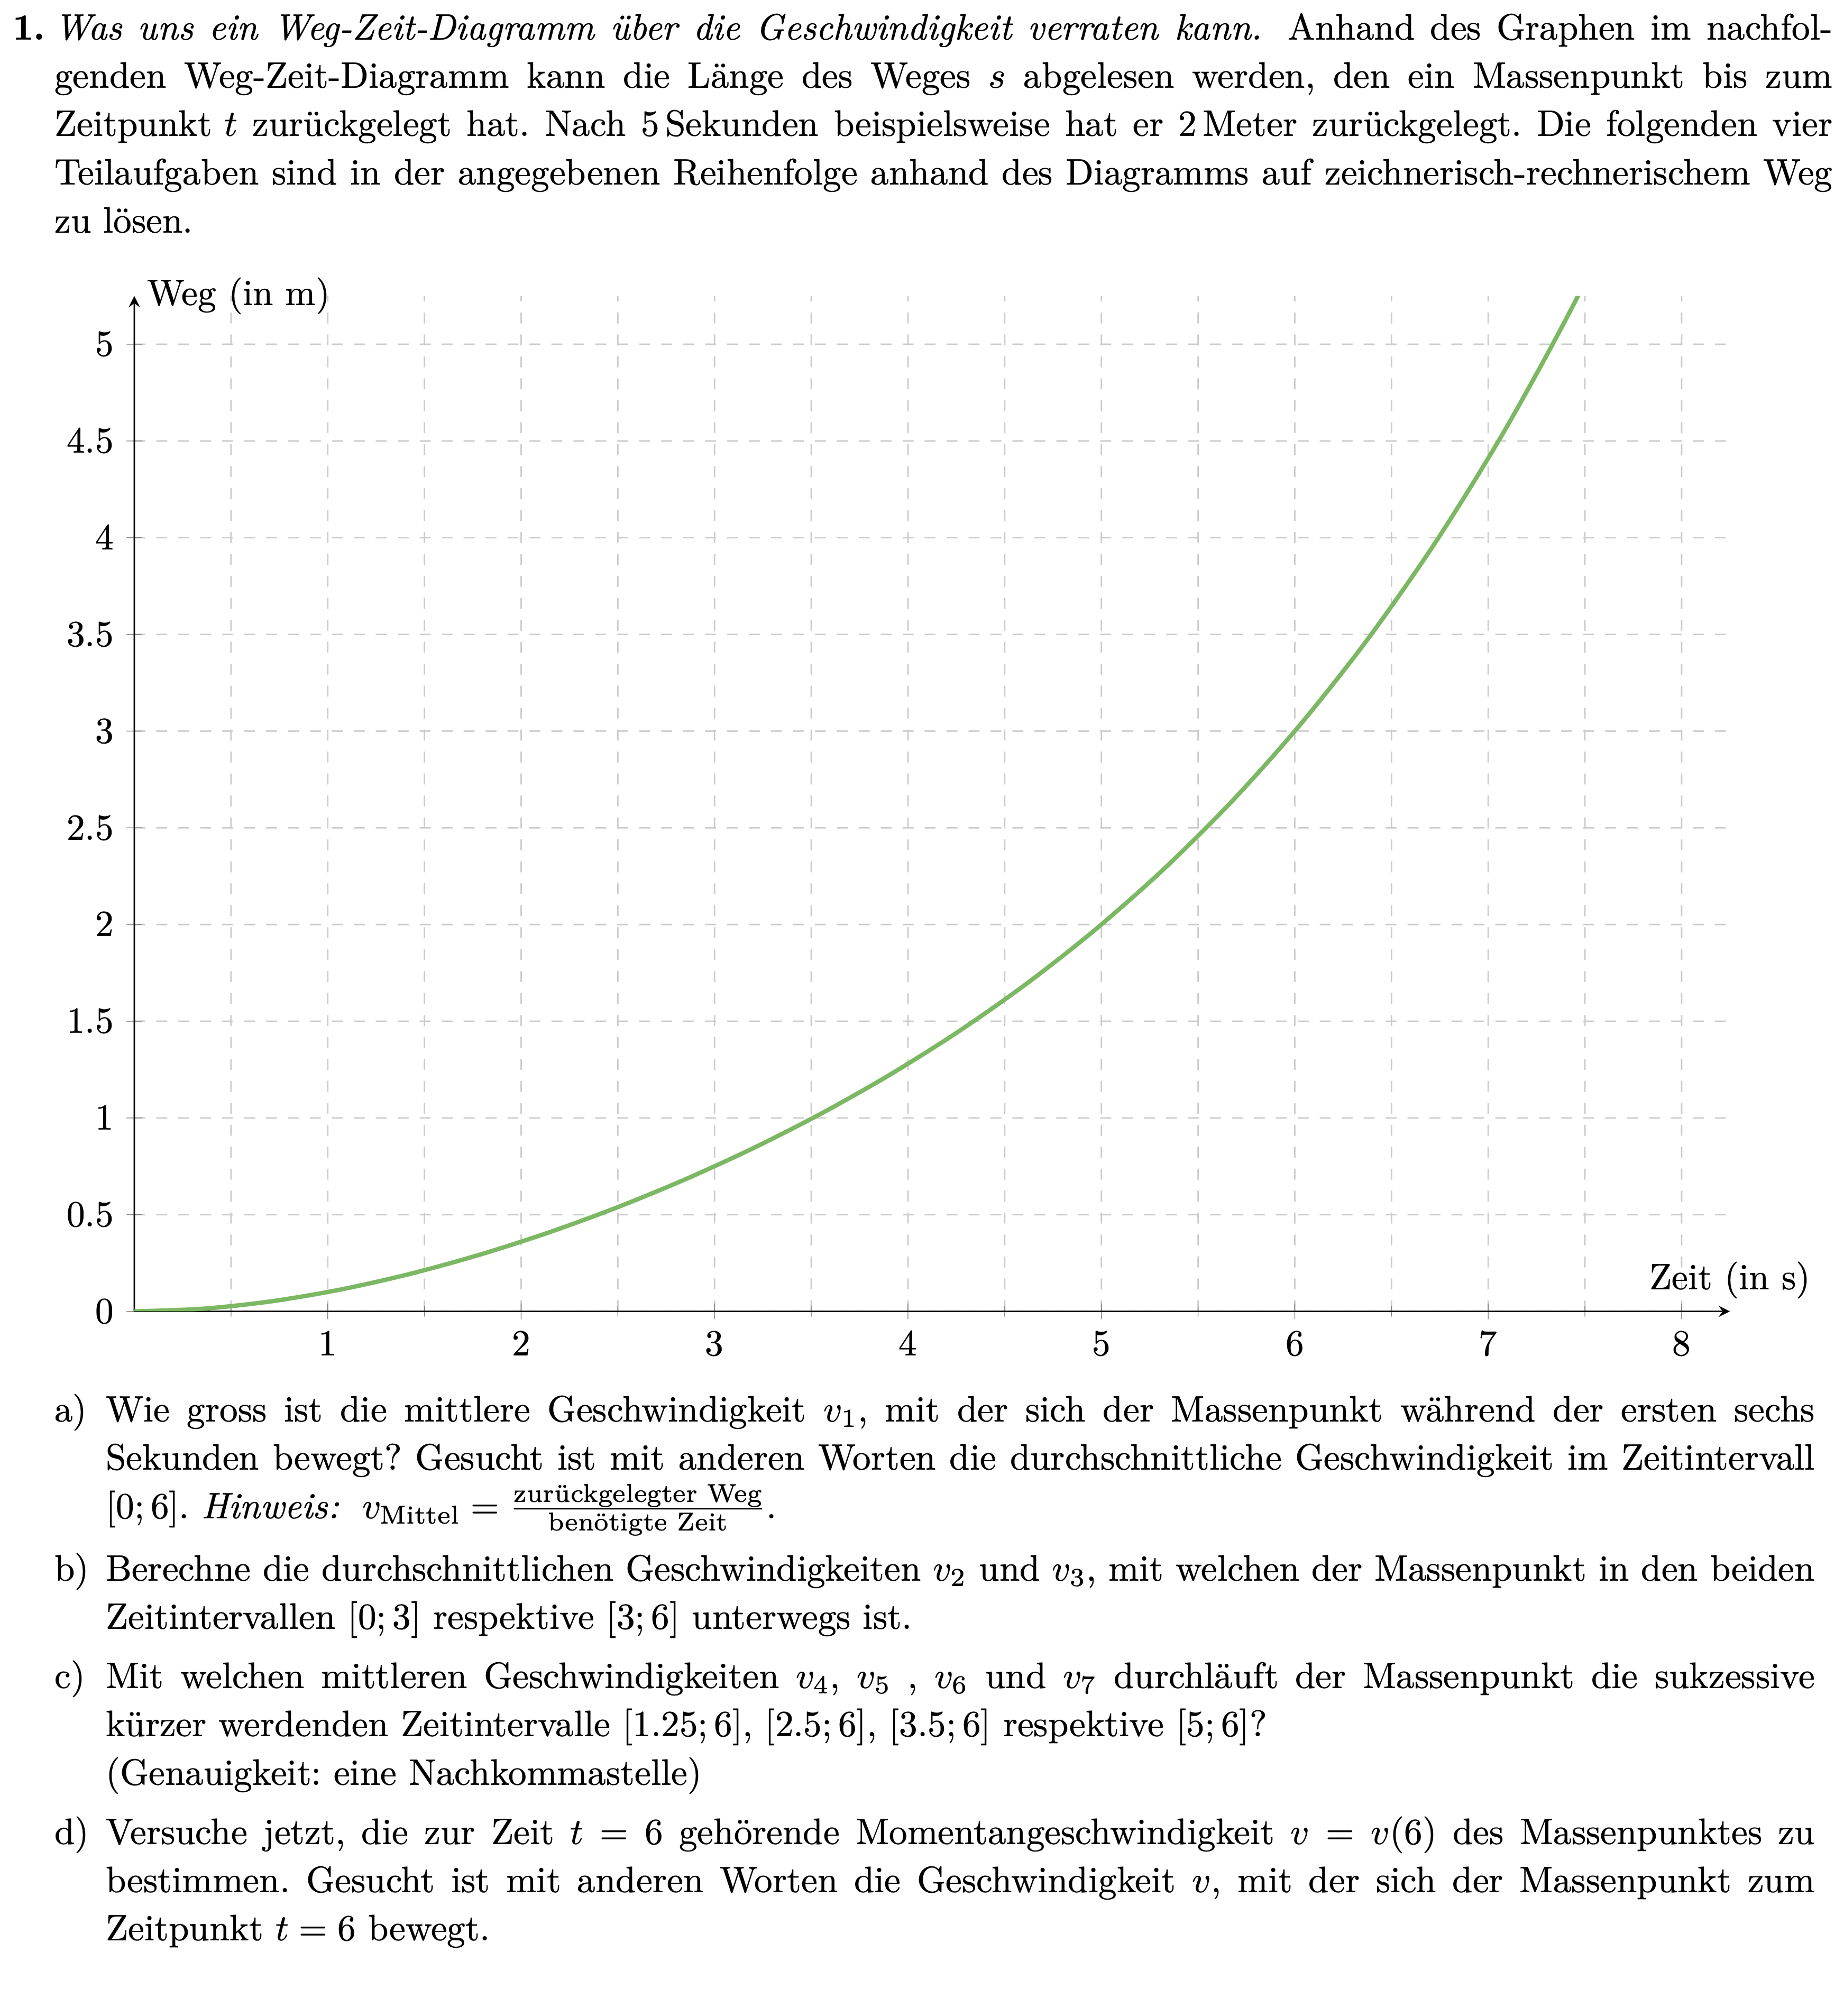
\includegraphics[scale=0.9]{media/AnalysisArbeitsblatt3-1-Aufgabe1.png}
    
\end{center}
\newpage
\begin{center}
    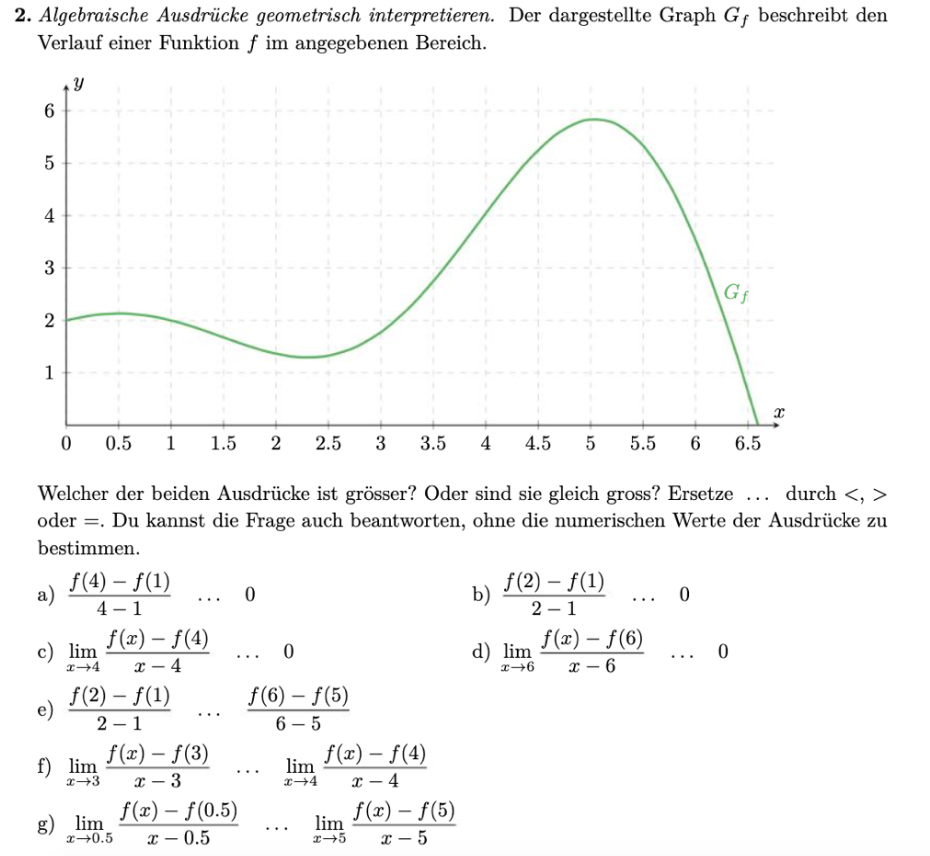
\includegraphics[scale=0.45]{media/Analysis3-1-Aufgabe2.png}
\end{center}
\begin{center}
    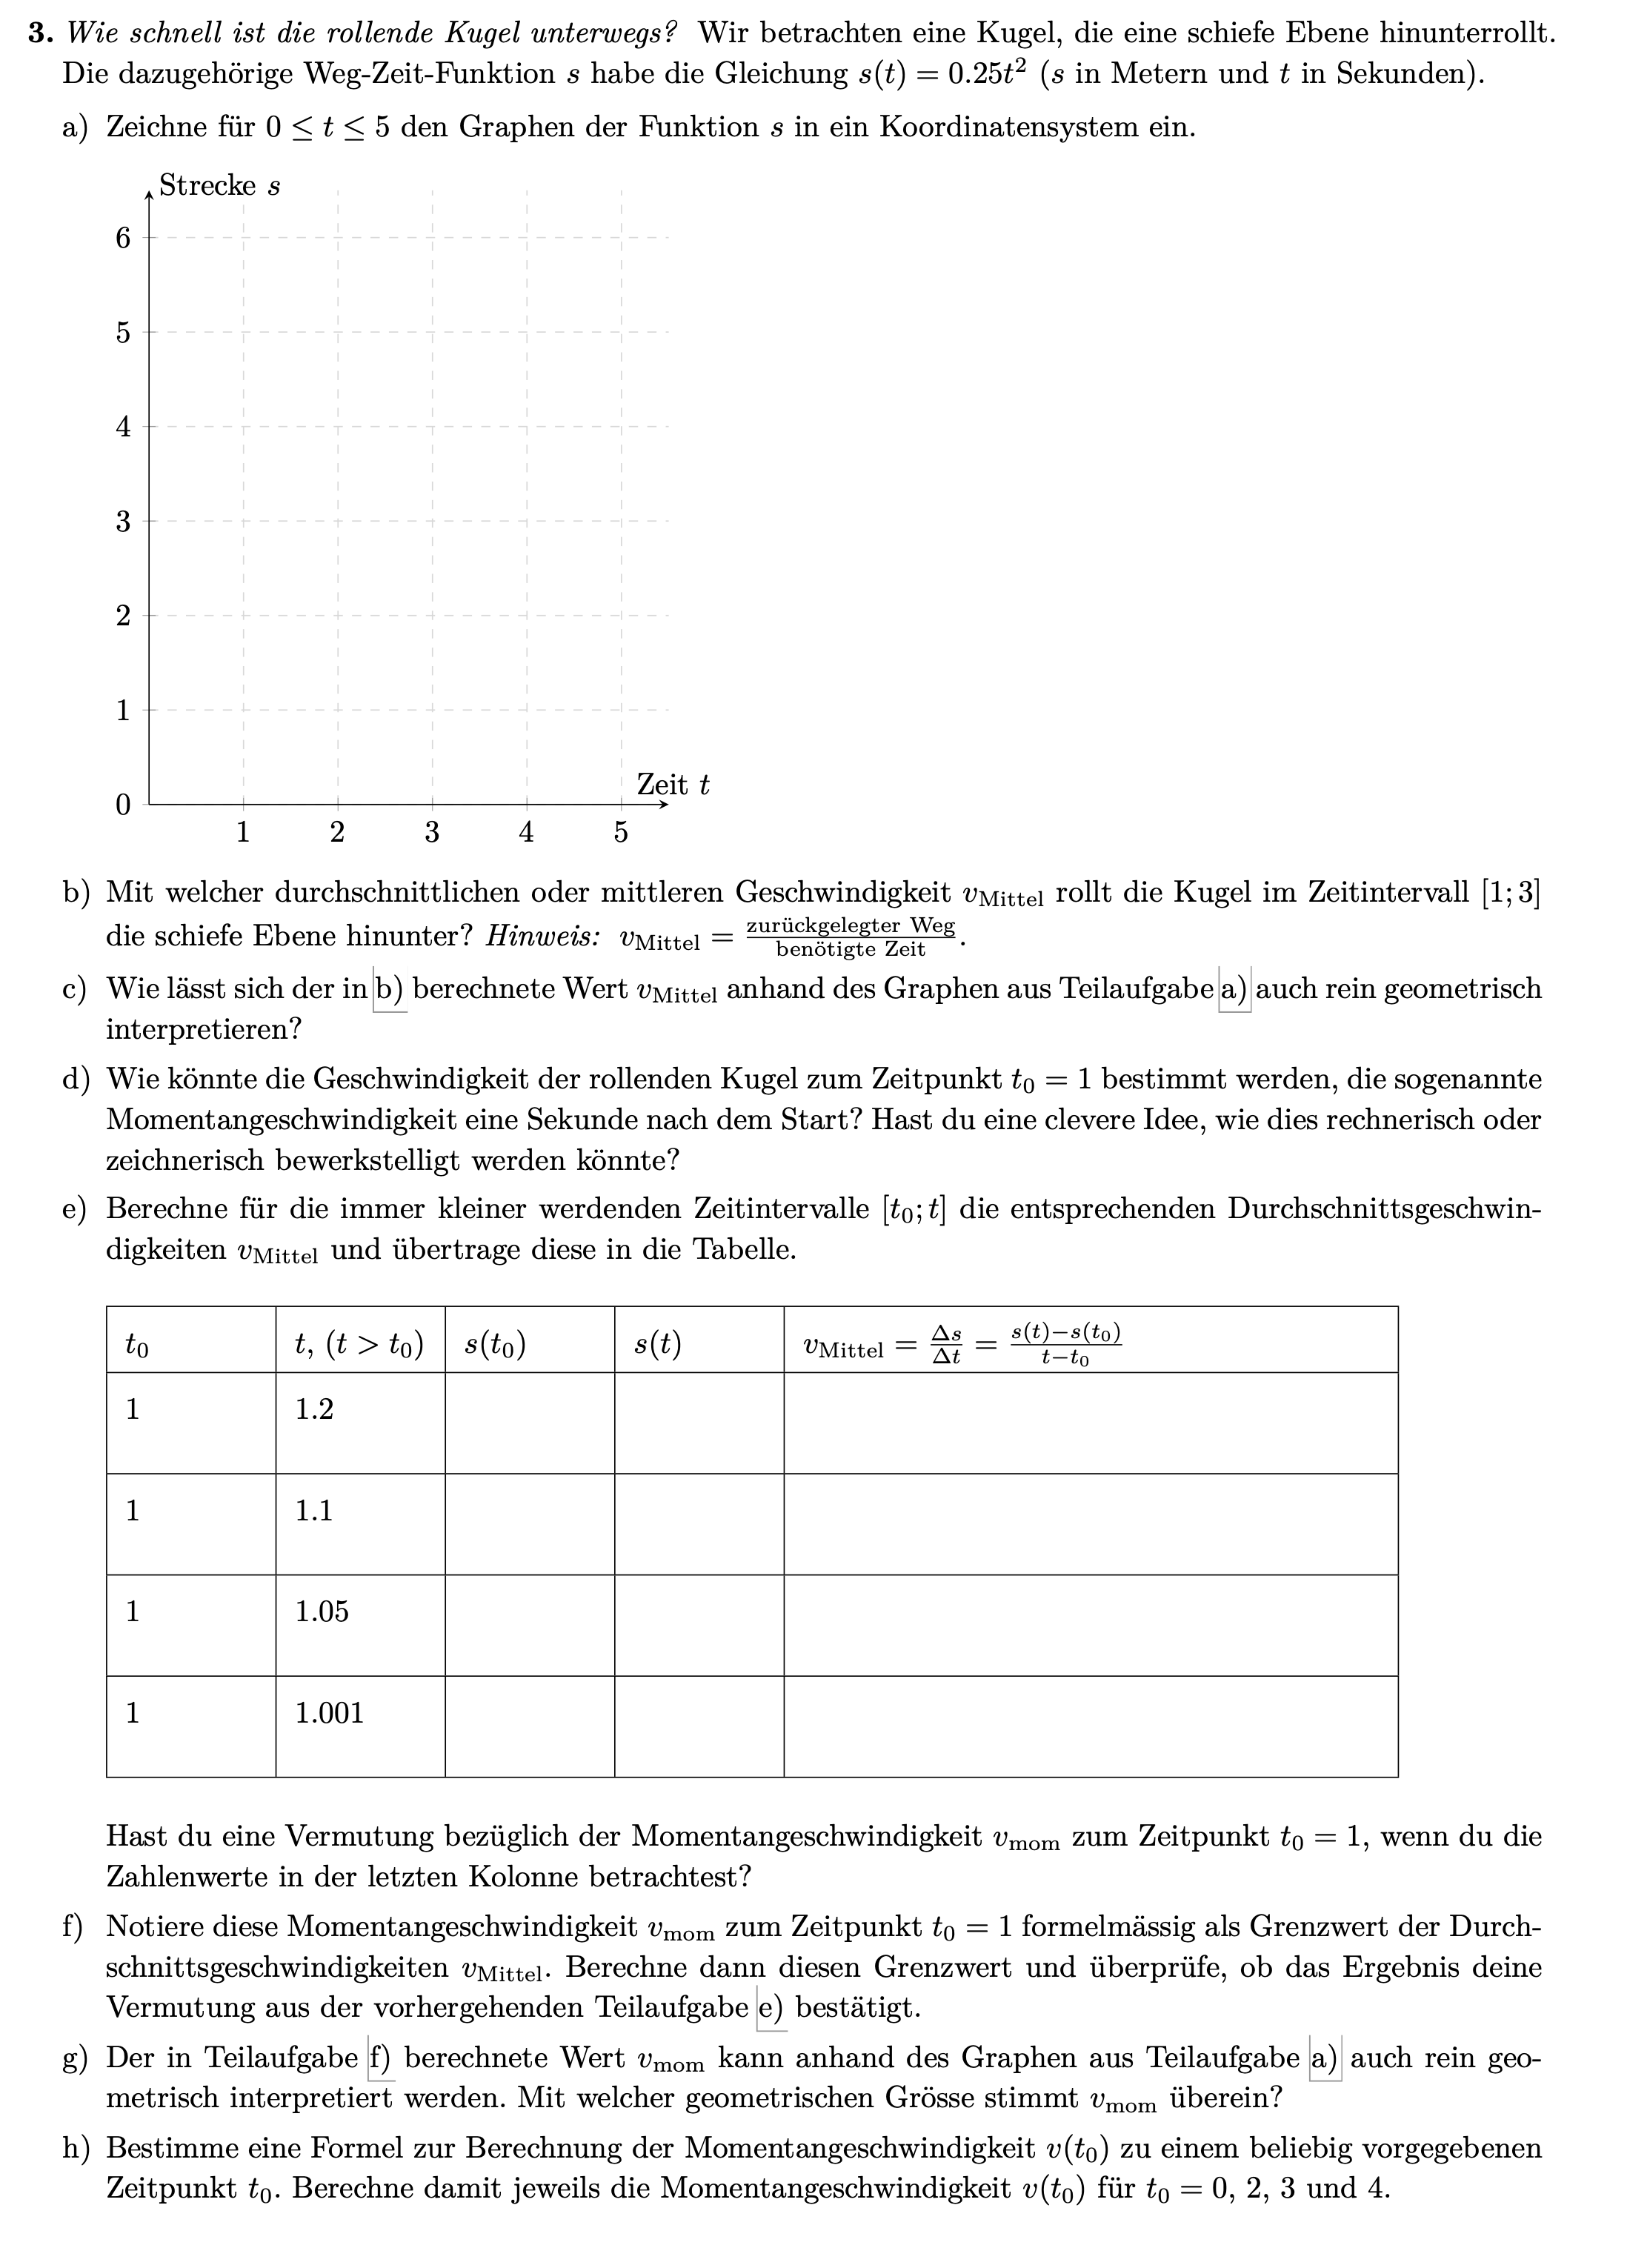
\includegraphics[scale=0.9]{media/AnalysisArbeitsblatt3-1-Aufgabe3.png}
\end{center}
\clearpage
In den drei Einführungsaufgaben haben Sie häufig Terme der Form $\frac{f(b)-f(a)}{b-a}$ untersucht, wobei Sie damit in Aufgabe 1 und 3 jeweils die mittlere Geschwindigkeit eines Objektes im Intervall $[a,b]$ berechnet haben. Vielleicht ist Ihnen in Aufgabe 2 aufgefallen, dass dieser Term auch die Steigung einer Geraden beschreibt, welche den Graphen von $f$ an den Stellen $x=a$ und $x=b$ schneidet. 

Je nach Kontext kann dieser Term auch eine mittlere Beschleunigung, Reaktionsgeschwindigkeit, Temperaturänderung und vieles mehr beschreiben (siehe auch die kommenden Aufgaben). Etwas allgemeiner gesprochen wird damit immer eine \emph{mittlere Änderungsrate} berechnet.

\begin{definition}
    {Differenzenquotient}{}
    Zu einer gegebenen Funktion und zwei verschiedenen Stellen $a$ und $b$ heisst der Term 
    $$\frac{\Delta y}{\Delta x} = \frac{f(b)-f(a)}{b-a} $$
    \emph{Differenzenquotient} oder \emph{mittlere Änderungsrate} der Funktion $f$ im Intervall $[a, b]$.

    Geometrisch entspricht der Differenzenquotient der Steigung der Sekanten, welche den Graphen von $f$ an den Stelle $x=a$ und $x=b$ schneidet.


     

    \begin{center}
        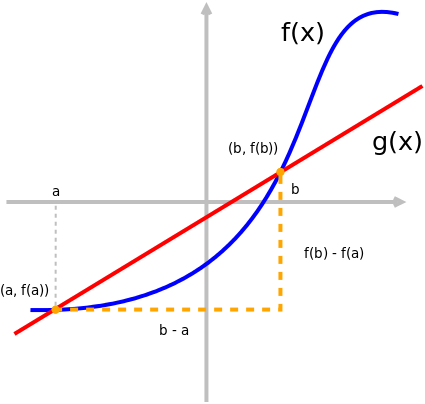
\includegraphics[scale=0.5]{media/differenzenquotient-graph.png}
    \end{center}
    Der Grenzwert $$\lim_{\Delta x \rightarrow0} \frac{\Delta y}{\Delta x}$$ nennt man \emph{momentane (oder lokale) Änderungsrate}. 
\end{definition}
\begin{ueb}{Zum Differenzenquotient}{}
    DMK Analysis ab Seite 52: \newline Zur Ermittlung des Differenzenquotienten: Aufgabe 4 und 5 \newline
    Zur Bedeutung des Differenzenquotienten: Aufgaben 6 bis 12
\end{ueb}

\clearpage

Mit dem Differenzenquotienten kann man aus der Weg-Zeit-Funktion die \emph{mittlere} Geschwindigkeit eines Objektes berechnen. Wie steht es aber mit der \emph{momentanen} Geschwindigkeit?

\begin{LA}
    {}{}
    Lösen Sie die Aufgabe 13 im Buch auf Seite 54
\end{LA}


\begin{definition}
    {Differentialquotient - Ableitung - momentane Änderungsrate}
    {}
    Falls der Grenzwert
$$\lim_{h\rightarrow0}\frac{f(x_0+h)-f(x_0)}{h}$$
existiert, so nennt man ihn \emph{Differenzialquotient oder (erste) Ableitung oder momentane (oder lokale) Änderungsrate der Funktion $f$ an der Stelle $x_0$}.

Bezeichnungen:
$$f'(x_0)   \text{ oder }  \frac{d}{dx} f(x_0)$$
Gesprochen: \glqq $f$ strich von $x_0$\grqq{} oder \glqq $df$ nach $dx$ an der Stelle $x_0$\grqq{}.

Geometrisch entspricht die Ableitung der Funktion an der Stelle $x_0$ der Steigung der Tangente, welche den Graphen von $f$ im Punkt $(x_0 | f(x_0))$ berührt.

\begin{center}
    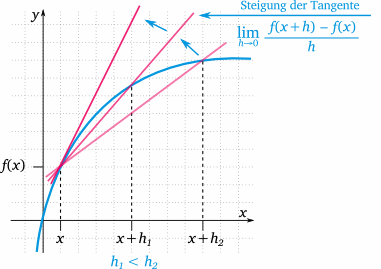
\includegraphics[]{media/tangente02-3.png}
\end{center}

\end{definition}



\begin{bsp}
    {Berechnung des Differentialquotienten}{}
    Gegeben sei die Funktion $f(x)=\frac{1}{2}x^2-x$. Gesucht ist die Ableitung von $f$ an der Stelle $x_0=5$

    %\vspace{7cm}

    Als erstes bestimmen wir den Differenzenquotienten:
    \begin{align*}
       \frac{\Delta y}{\Delta x} &= \frac{f(5+h)-f(5)}{h} \\
       &= \frac{\left(\frac{1}{2} (5+h)^2-(5+h) \right) - \left(\frac{1}{2}5^2 -5 \right)}{h} \\
       %&= \frac{\left(\frac{1}{2}(25+10h+h^2)\right)-\frac{15}{2}}{h} //
       &= \frac{\frac{1}{2}h^2+4h}{h}
    \end{align*}
    Anschliessend bilden wir den Grenzwert für $h\rightarrow0$:
    $$f'(5) = \lim_{h\rightarrow0}\frac{\Delta y}{\Delta x}= \lim_{h\rightarrow0} \frac{\frac{1}{2}h^2+4h}{h} = \lim_{h\rightarrow0}\left(\frac{1}{2}h+4\right) = 4$$
\end{bsp}
\begin{ueb}
    {}{}
    Aufgaben im Buch auf Seite 55: 16 bis 20
\end{ueb}
Nach den Erkenntnissen aus dem Kapitel über Grenzwerte wissen wir, dass diese nicht immer existieren. Somit kann es auch sein, dass für eine gegebene Funktion den Differentialquotienten an einer bestimmten Stelle gar nicht gebildet werden kann.
\begin{definition}
    {Differenzierbarkeit}{}
    Sei $f$ eine beliebige Funktion und $x_0 \in \mathbb{D}_f$. Falls der Grenzwert 
    $$ \lim_{h\rightarrow0}\frac{f(x_0+h)-f(x_0)}{h} $$
    existiert, so sagt man, dass die Funktion $f$ an der Stelle $x_0$ \emph{differenzierbar} ist.
\end{definition}

Die Betragsfunktion $x\mapsto |x|$ ist beispielsweise überall differenzierbar mit Ausnahme der Stelle $x_0$.
\begin{center}
    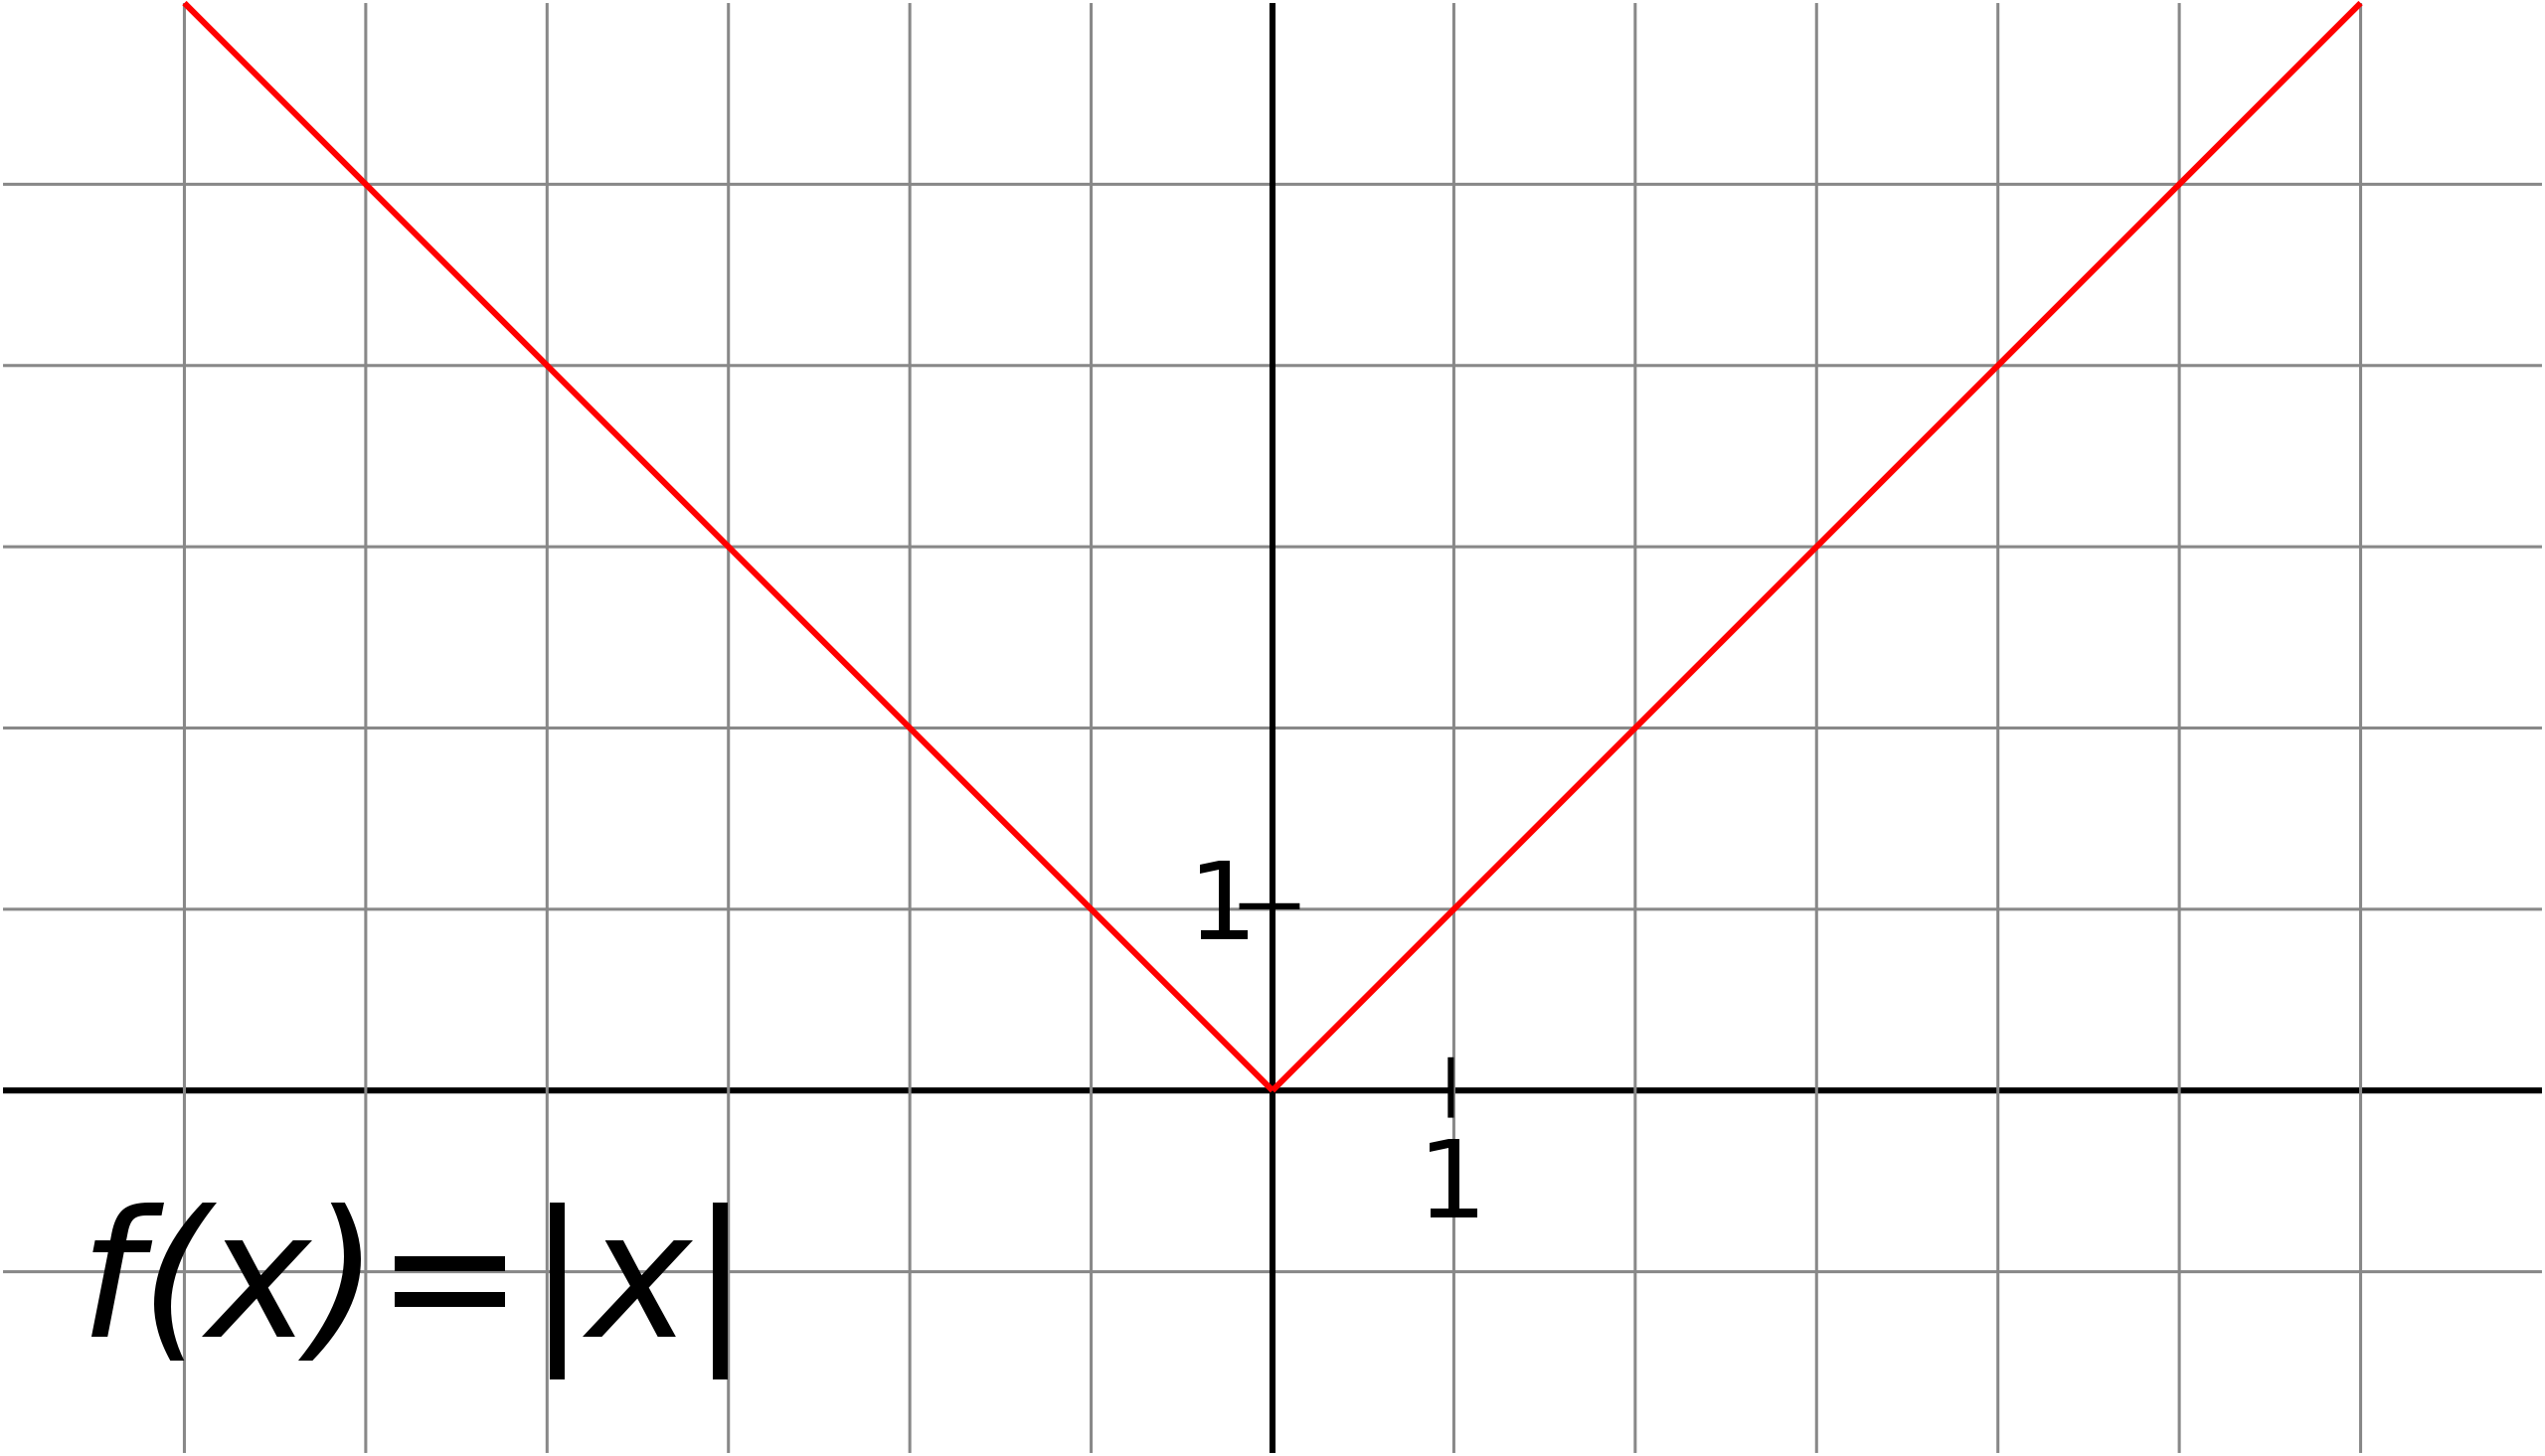
\includegraphics[scale=0.1]{media/Abs(x).png}
\end{center}
Schätzen Sie: Was wären in diesem Fall der links- bzw. rechtsseitige Grenzwert $\lim_{\Delta x\uparrow 0} \frac{\Delta y}{\Delta x}$ und $\lim_{\Delta x\downarrow 0} \frac{\Delta y}{\Delta x}$?

Wenn die Funktion überall differenzierbar ist, kann in jedem Punkt des Graphen die Steigung der Tangente ermittelt werden. Die Zuordnung \emph{
$x\mapsto$ Steigung des Graphen von $f$ an der Stelle $x$} ist wieder eine Funktion!

\begin{definition}
    {Ableitungsfunktion}{}
    Gegeben sei eine differenzierbare Funktion $f$. Die Funktion mit der Zuordnungsvorschrift:
    $$x\mapsto f'(x)=\lim_{h\rightarrow0}\frac{f(x+h)-f(x)}{h}$$
    heisst die \emph{Ableitungsfunktion} (kurz: \emph{die Ableitung}) der Funktion $f$. Sie wird mit $f'$ bezeichnet. 
    \newline
    Geometrisch interpretiert beschreibt der Output von $f'$ die Steigung der Tangente an den Graphen von $f$ im Punkt $(x|f(x))$.
  
\end{definition}

\begin{bsp}
    {Berechnung der Ableitungsfunktion}{}
    Sei $f(x)=x^2+1$. Die Gleichung der Ableitungsfunktion kann wie folgt hergeleitet werden:
    \begin{align*}
        f'(x)   &= \lim_{h\rightarrow0}\frac{f(x+h)-f(x)}{h}\\
                &=  \lim_{h\rightarrow0}\frac{\left((x+h)^2+1\right)-\left(x^2+1\right)}{h}\\
                &= \lim_{h\rightarrow0}\frac{\left(x^2+2hx+h^2+1\right)-\left(x^2+1\right)}{h}\\
                &= \lim_{h\rightarrow0}\frac{2hx+h^2}{h}\\
                &= \lim_{h\rightarrow0}\left(2x+h\right)\\
                &= 2x
    \end{align*}
    Die erste Ableitung von $f$ ist damit $f'(x)=2x$. In anderen Worten: Die Tangente, welche den Graphen von $y=x^2+1$ an der Stelle $x$ berührt hat die Steigung $2x$.
    So hat die Tangente an $y=x^2+1$ an der Stelle $x=5$ die Steigung $f'(5)=10$.
    
\end{bsp}
\begin{ueb}
    {}{}
    Im Buch auf Seite 56: 21 und 25-27
\end{ueb}

